% AIAA SciTech Forum conference paper -- DRAFT
%
% Build:  pdflatex paper && bibtex paper && pdflatex paper && pdflatex paper
% Class/style files live in style/ -- either compile with
%   TEXINPUTS=./style: BSTINPUTS=./style: pdflatex paper
% or copy aiaa-tc.cls and aiaa.bst next to this file.
%
% NOTE: style/aiaa-tc.cls and style/aiaa.bst were hand-extracted from the
% CTAN docstrip sources -- regenerate with `latex aiaa.ins` before a real
% submission (see README.md).

\documentclass[]{aiaa-tc}% conference mode (10pt); insert '[draft]' to show overfull boxes

\usepackage[utf8]{inputenc}
\usepackage{amsmath}
\usepackage{url}

\title{Vectored Thrust of a Ducted Fan with Jet Vanes by a\\
       Two-Way Coupled Rotating-Frame Vortex Lattice Method}

\author{
 Onur Tuncer%
  \thanks{TODO: job title, department, address, AIAA member grade.}\\
 {\normalsize\itshape
  TODO: affiliation, city, country}
}

% Data used by 'handcarry' option if invoked
\AIAApapernumber{TODO-YEAR-NUMBER}
\AIAAconference{AIAA SciTech Forum, TODO date and location}
\AIAAcopyright{\AIAAcopyrightD{TODO-YEAR}}

\newcommand{\eqnref}[1]{(\ref{#1})}

\begin{document}

\maketitle

\begin{abstract}
Control of a ducted-fan VTOL aircraft at hover rests on vanes immersed
in the propulsor's own jet: at zero airspeed the propwash is the only
dynamic pressure available to them. This paper presents a
potential-flow method that resolves the complete propulsive wrench of
such a system --- rotor, duct, and exit vanes --- in seconds per
operating point. The rotor is solved as a vortex lattice in the
blade-fixed rotating frame, with blades meshed on their CST camber
surfaces wrapped on radius cylinders and trailing legs prescribed along
the local relative wind, which keeps the hover limit well posed. The
duct is paneled into the same solve as constant-strength source rings,
a two-way interaction converged with the blade circulation. The exit
vanes cannot share the rotating frame; they are solved in the inertial
frame, reading the rotor through a time-mean slipstream reconstructed
from the converged radial loading by annular momentum theory, with a
viscous sectional coupling that handles their separation-dominated
hover aerodynamics. A block Gauss--Seidel alternation closes the loop
between the two frames, constrained by a swirl momentum budget: the
vanes cannot extract more torque than the jet's angular-momentum flux
--- the shaft torque --- delivers. On a reference cruciform
configuration at hover the budget binds, the vanes recovering 99\% of
the available angular momentum where an uncoupled scheme reported three
times that, and the converged control response about neutral is nearly
antisymmetric. The method is implemented in the open-source C++23
toolkit Aeolion.
\end{abstract}

\section*{Nomenclature}

\begin{tabbing}
  XXXXXXX \= \kill% this line sets tab stop
  $c$        \> section chord \\
  $c_l$      \> section lift coefficient \\
  $M_x$      \> rolling moment about the rotation axis \\
  $p$        \> body-axis roll rate \\
  $Q$        \> shaft torque \\
  $q$        \> dynamic pressure \\
  $r$        \> radial station \\
  $R$        \> rotor tip radius \\
  $s$        \> swirl budget factor \\
  $T$        \> thrust \\
  $v_i$      \> annulus axial induced velocity \\
  $V_{ax}$   \> axial onset velocity at the disk \\
  $V_{kin}$  \> kinematic (rotational + freestream) local velocity \\
  $V_{rel}$  \> local relative velocity \\
  $w_i$      \> annulus swirl velocity \\
  $\alpha_{eff}$ \> effective section angle of attack \\
  $\Gamma$   \> bound circulation \\
  $\lambda$  \> inflow ratio \\
  $\sigma$   \> source panel strength \\
  $\Omega$   \> rotor angular speed \\[5pt]
  \textit{Subscripts}\\
  $i$ \> radial strip index \\
 \end{tabbing}

\section{Introduction}

% TODO: expand with VTOL/ducted-fan literature review and citations
% (ducted-fan tail-sitters, jet-vane control, swirl-recovery vanes).

Tail-sitter VTOL aircraft of the ducted-fan class obtain control at
hover from vanes placed in the duct's exit jet. Their sizing question
is awkward for the established toolchain: at zero airspeed a
conventional vortex lattice or panel method has no freestream dynamic
pressure to put on a control surface, so vane authority, the thrust
cost of vectoring, and the recovered swirl torque are outside such
tools' model entirely, while RANS CFD of the full rotor--duct--vane
system is too slow for the configuration loop. Classical VLM codes
such as AVL~\cite{avl} treat the airframe with, at most, a prescribed
actuator-disk propulsor; isolated-rotor methods such as
XROTOR~\cite{xrotor} carry no airframe and no vanes.

This paper describes a method that closes that gap at
potential-flow-plus-sectional-viscous fidelity, resolving the coupled
rotor--duct--vane system in seconds. Three ingredients are presented
in turn: the rotating-frame vortex lattice for the rotor
(Sec.~\ref{s:rotor}), the two-way ducted solve and the inertial-frame
vane solve with its reconstructed slipstream (Secs.~\ref{s:duct},
\ref{s:vanes}), and the two-way rotor--vane alternation with its swirl
momentum budget (Sec.~\ref{s:coupling}). Results on a reference
cruciform configuration at hover follow in Sec.~\ref{s:results}. The
method is implemented in Aeolion, an open-source C++23 aerodynamics
toolkit; the mathematical elements --- horseshoe vortices and
constant-strength source panels --- are the textbook
ones~\cite{katzPlotkin2001}, and the contribution is the coupling.

\section{Rotor: Vortex Lattice in the Rotating Frame}
\label{s:rotor}

The rotor is the same vortex lattice as a wing, posed in the
blade-fixed rotating frame. Rotation is not special-cased in the
solver: it enters as the body roll rate $p = \Omega$, whose kinematic
velocity $\mathbf{V}_{kin} = \mathbf{V}_\infty -
\boldsymbol{\omega} \times \mathbf{r}$ hands every blade panel its
true $\Omega r$ tangential onset flow. The near-field
Kutta--Joukowski force evaluation uses that same local velocity, so
the body-axis load sums are dimensional propeller loads directly:
thrust $T = -F_x$, shaft torque $Q = -M_x$, power $P = Q\,\Omega$.

Each blade is meshed with one Weissinger row per radial strip on the
blade's CST camber surface~\cite{kulfan2008}, with two geometric
choices that proved load-bearing rather than cosmetic:

\begin{enumerate}
\item \emph{Chords wrap on their radius cylinders} --- the surface a
blade element actually sweeps --- rather than lying in a flat tangent
plane. Near a small hub, where chord is comparable to radius, a
tangent-plane chord subtends tens of degrees of azimuth, and the
phantom incidence it picks up can overwhelm the real camber and twist
loading.
\item \emph{Trailing legs leave along the local relative wind} at
their roots --- the tangential sweep plus the axial inflow, floored at
the momentum-theory hover inflow $\lambda \approx 0.07$ --- a
prescribed linearized helix. At hover the local wind is almost purely
tangential: trailing the wake axially instead leaves the legs
near-perpendicular to the flow and the circulation solve diverges
under refinement, while without the inflow floor a straight tangential
leg lies in the rotor plane forever, crossing every radius outboard of
its root.
\end{enumerate}

The bare lattice is quasi-steady with a prescribed straight-line wake
(no roll-up or contraction), carries induced torque only, and has no
stall. The last two limitations are removed by a sectional
viscous--inviscid coupling: per radial strip, the lattice provides
$\alpha_{eff}$ from the local kinematic-plus-induced velocity, a 2-D
section model provides $c_l(\alpha_{eff}, Re, Ma)$, the target
circulation follows from the Kutta--Joukowski relation
$|\Gamma| = \tfrac{1}{2} V_{rel}\, c\, c_l$, and the fixed point
\begin{equation}
 \label{e:residual}
 R_i(\Gamma) = c_{l,i}^{VLM}(\Gamma)
   - c_{l,i}^{sect}\!\bigl(\alpha_{eff,i}(\Gamma), Re_i, Ma_i\bigr) = 0
\end{equation}
is converged with type-II Anderson acceleration~\cite{anderson1965}
(67 plain-relaxation iterations reduced to 9 on the reference rotor),
guarded by a kinematic-speed circulation cap that breaks the
$\Gamma \to V_{rel} \to \Gamma$ runaway. The section model is an
interface seam: an analytic viscous polar, or a transpiration-coupled
integral boundary-layer solver (Thwaites~\cite{thwaites1949},
Head~\cite{head1958}, Squire--Young~\cite{squireYoung1938}) whose
displacement effect enters the 2-D section problem as transpiration
boundary conditions. The coupling caps the stalled hover root loading
the inviscid lattice overpredicts and puts profile torque into the
shaft-power sum.

\section{The Ducted Rotor}
\label{s:duct}

The duct is meshed as a closed annular ring of constant-strength
source panels (outer wall, bore wall, two caps) centered on the rotor
plane, and passed into the coupled solve as its source system. The
interaction is two-way: every coupling iteration re-solves the source
strengths against the current blade circulation (the duct's
no-through-flow condition sees the propwash; the source-only influence
block is factored once), and the strip velocities include the duct's
induced flow (the blades see the bore's constriction). One frame
subtlety makes this legitimate: in the blade-fixed frame the duct
rotates backwards, but a body of revolution about the rotation axis
moves only tangentially to itself, so its boundary condition is
unchanged (exactly, up to sector faceting).

The duct's own load is the surface-pressure integral
$\mathbf{F} = \sum (\tfrac{1}{2}\rho |V|^2 - q_\infty) A\,
\hat{\mathbf{n}}$, well behaved at hover where the gauge $q_\infty$ is
negligible --- and this is where a shroud earns its keep: the
bore-lip suction ahead of the disk points upstream.

\section{Exit Vanes and the Reconstructed Slipstream}
\label{s:vanes}

The exit vanes are all-moving flat plates at the duct exit, spanning
radially on their hinge axes and deflecting as rigid rotations about
them. They cannot share the rotor's frame: a non-axisymmetric surface
swept backwards through a rotating frame has a time-dependent boundary
condition. The solve is therefore partitioned by frame --- the vanes
are meshed as ordinary lifting surfaces and solved in the inertial
frame ($p = 0$), reading the rotor system through a prescribed
external slipstream.

That slipstream is \emph{reconstructed}, not field-averaged. The
quasi-steady rotor's prescribed straight trailing legs never wrap into
the downstream helical wake cylinder, so their Biot--Savart mean
carries swirl but almost no axial jet a few chords aft of the disk;
vanes placed there would see no dynamic pressure. Instead, annular
momentum theory is applied to the loads the lattice actually
converged: per annulus,
\begin{equation}
 \label{e:slipstream}
 dT = 4\pi r \rho\, (V_{ax} + v_i)\, v_i \, dr
 \;\Rightarrow\; v_i ,
 \qquad
 dQ = 4\pi r^3 \rho\, (V_{ax} + v_i)\, w_i \, dr
 \;\Rightarrow\; w_i ,
\end{equation}
with $dT$, $dQ$ summed over blades from the per-strip forces, the
axial component developing toward the classical far-wake doubling over
about a diameter, the swirl carried unchanged, and the duct's exact
source induction added on top.

The vanes receive the same viscous sectional coupling as the blades,
with the boundary-layer section model by default and each trailing leg
leaving along the \emph{local mean flow} at its root --- in the jet,
helically, with the swirl. This matters twice over. First, at hover
the swirl alone puts the vanes near $16$--$20^\circ$ of local
incidence before any command, so their hover aerodynamics are
separation-dominated by nature; the section solver resolves attached
and mildly separated flow, blends into a saturated polar, and applies
a flat-plate deep-stall decay beyond it. Second, two numerical
safeguards proved necessary: the coupling residual is weighted by
local dynamic pressure (a vane tip parked at $85^\circ$ incidence in
the jet's shear edge at 7\% of the jet's $q$ must not hold the solve
hostage), and the deep-stall decay is what makes such strips
satisfiable at all.

The propulsive wrench is the sum of the two solves' near-field loads
about the hub: rotor circulatory and profile forces, duct surface
pressure, vane circulatory and profile forces. The vanes' drag debits
the net thrust; their side forces and $M_y/M_z$ are the control
authority --- real at zero airspeed, the propwash being their only
dynamic pressure --- and even undeflected they recover part of the
swirl as counter-torque.

\section{Two-Way Coupling and the Swirl Momentum Budget}
\label{s:coupling}

Partitioned as above, the scheme is one-way: the vanes read the jet,
the rotor never feels the vanes, and nothing depletes the prescribed
swirl --- a high-solidity vane set can recover more torque than the
jet carries. The two-way scheme closes the loop as a block
Gauss--Seidel alternation between the frames. Per outer pass:

\begin{enumerate}
\item \emph{Rotor + duct solve} (rotating frame), with the vanes
entering through the external-velocity hook as the azimuthal mean of
their induced field,
\begin{equation}
 \label{e:meanfield}
 \bar{\mathbf{v}}_{vane}(P) = \frac{1}{K} \sum_{j=0}^{K-1}
   R_x(-\theta_j)\, \mathbf{v}_{vane}\bigl( R_x(\theta_j) P \bigr),
 \qquad \theta_j = 2\pi j / K .
\end{equation}
A blade sweeps past the static vane system once per revolution, and
its quasi-steady condition sees the time mean of that encounter.
Averaging is legitimate in \emph{this} direction because the vane
system's near field is fully represented by its explicit legs --- it
is exactly the operation that fails in the other direction.
\item \emph{Slipstream reconstruction} from the fresh rotor loading,
Eq.~\eqnref{e:slipstream}, with the swirl scaled by the budget factor
$s \in (0,1]$.
\item \emph{Vane remesh and solve} (inertial frame) --- remesh,
because the trailing legs follow the local mean flow, which just
changed.
\item \emph{The swirl budget.} The angular-momentum flux the jet
delivers is the shaft torque, $\dot{L}_{jet} = Q = -M_x^{rotor}$; the
vanes cannot remove more than arrives. Whenever the extracted
$M_x^{vane}$ exceeds it, the swirl factor contracts,
\begin{equation}
 \label{e:budget}
 s \;\leftarrow\; s \cdot \frac{Q}{M_x^{vane}} ,
\end{equation}
whose fixed point is the budget-saturated state
$M_x^{vane} = Q$ --- vanes that de-swirl the jet essentially
completely.
\item \emph{Relaxation and convergence.} The vane circulation fed back
to the rotor is under-relaxed; the outer residual is the relative
change of the total wrench together with the vane-circulation change.
\end{enumerate}

Still outside the model, by construction: unsteady blade-passing loads
(every exchange is a time mean), the vanes' straight-line wakes, and
radially resolved swirl depletion --- the budget is a single scalar,
the natural refinement being a band-by-band bookkeeping.

\section{Results}
\label{s:results}

% TODO: regenerate all numbers in this section from the current build
% and state the reference geometry (blade, duct, vane contract
% parameters) explicitly, ideally in a table.

Results are shown for a reference two-blade rotor with a snug shroud
(4\% tip clearance) and a four-vane cruciform at the duct exit, at
static (hover) conditions.

\paragraph{Ducted rotor.} At hover the shroud lifts thrust from
7.60~N open to 8.82~N ducted ($+16\%$), the duct itself carrying
$+1.17$~N of bore-lip suction, with the coupled solve converged in 9
iterations; the static comparison across rpm
(Fig.~\ref{f:ducted_vs_open}) shows the $\sim$15\% augmentation at
essentially unchanged shaft torque. A loosely fitted ring with large
tip clearance correctly earns almost nothing --- the augmentation is
the interaction, not the presence of a ring.

\begin{figure}[htb]
 \centering
 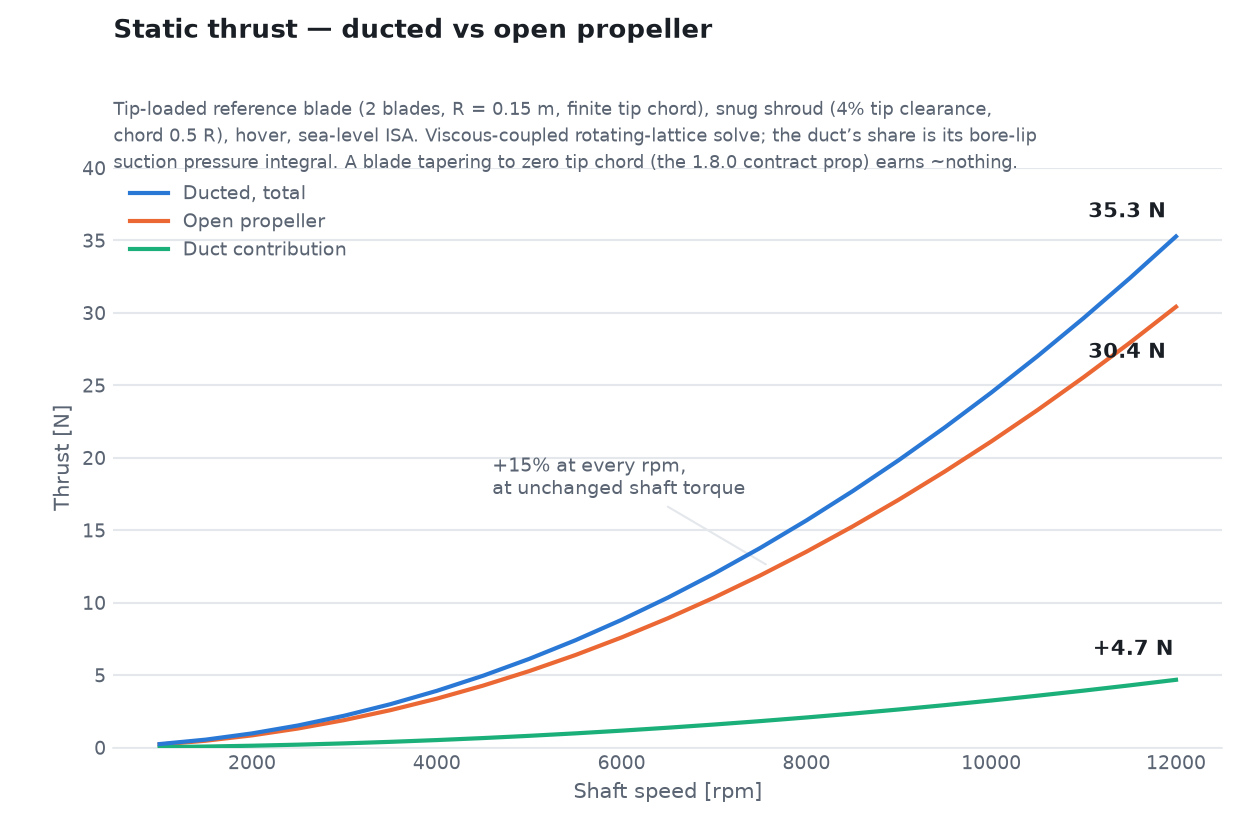
\includegraphics[width=0.75\textwidth]{figures/ducted_vs_open}
 \caption{Static thrust versus rpm, ducted versus open rotor, with the
   duct's own contribution shown separately.}
 \label{f:ducted_vs_open}
\end{figure}

\paragraph{Vane system and the budget.} On the reference cruciform at
hover the outer alternation converges in 7 passes. The swirl budget
binds hard: the swirl factor converges near $s = 0.33$, and the vanes
recover 99\% of the jet's angular-momentum flux --- the
budget-saturated, essentially complete de-swirl state --- where the
one-way scheme had reported three times the available torque. The
rotor measurably feels the vanes' blockage (a thrust shift, a
perturbation rather than an upheaval), and with the budgeted swirl
bias small, the control response about neutral is nearly
antisymmetric: $+0.100$~/~$-0.104$~N of side force at $\pm 8^\circ$
of vane deflection. Wake direction matters at this level: pointing
the vane wakes along the local mean flow (helically, with the swirl)
rather than hardcoded downstream roughly doubled the control response
about the swirl-biased neutral and strengthened the undeflected
counter-torque.

\begin{figure}[htb]
 \centering
 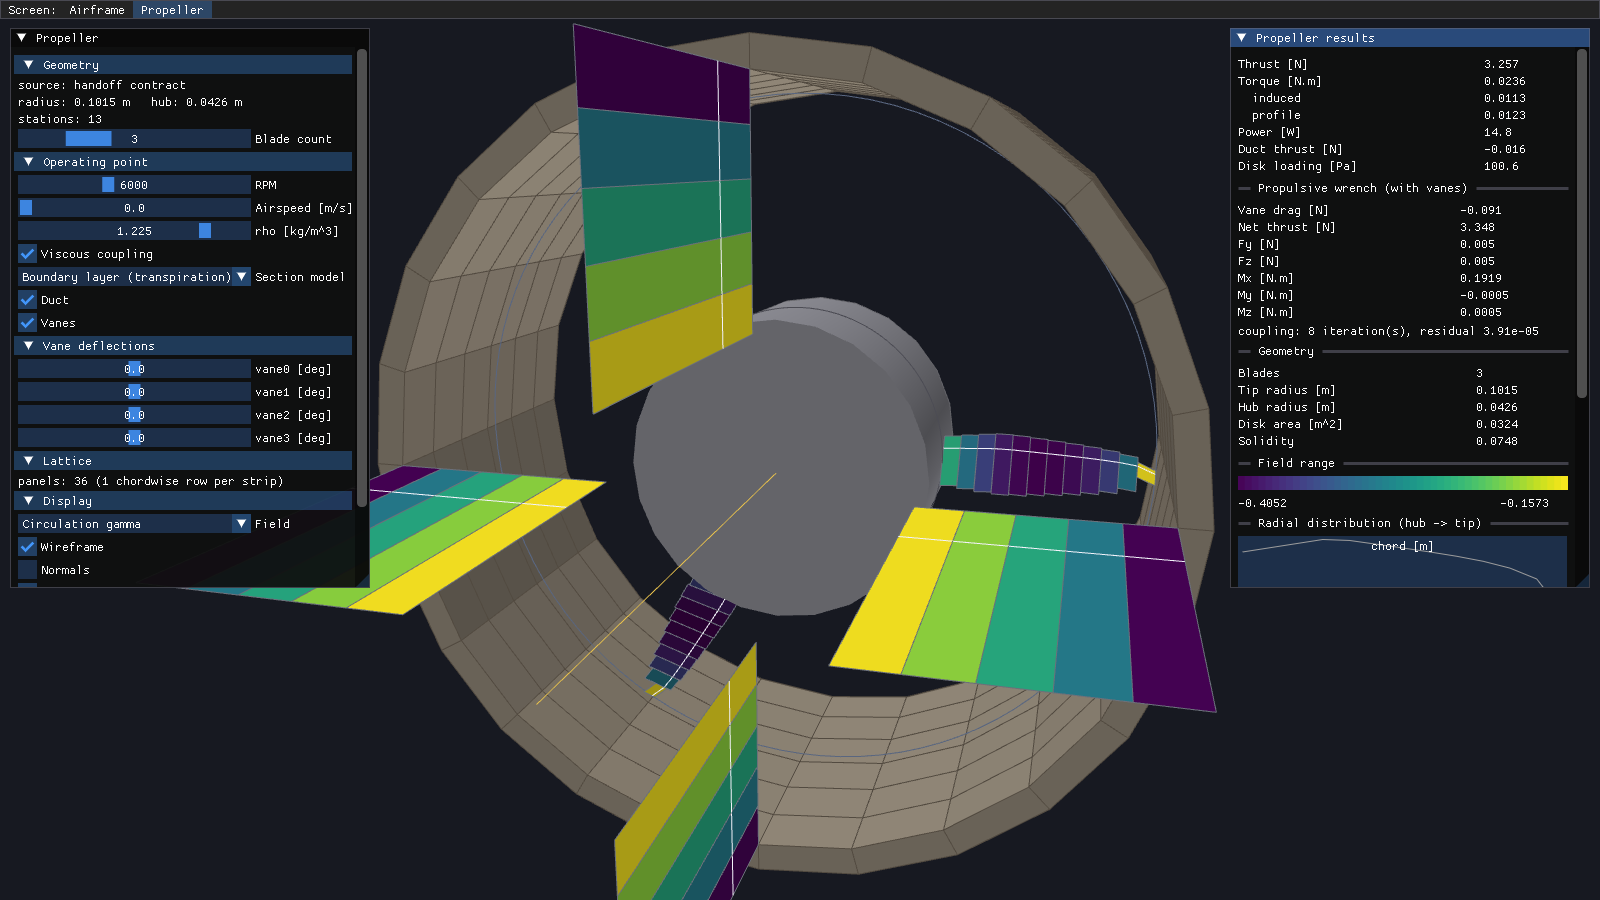
\includegraphics[width=0.48\textwidth]{figures/viewer_vanes_aft}\hfill
 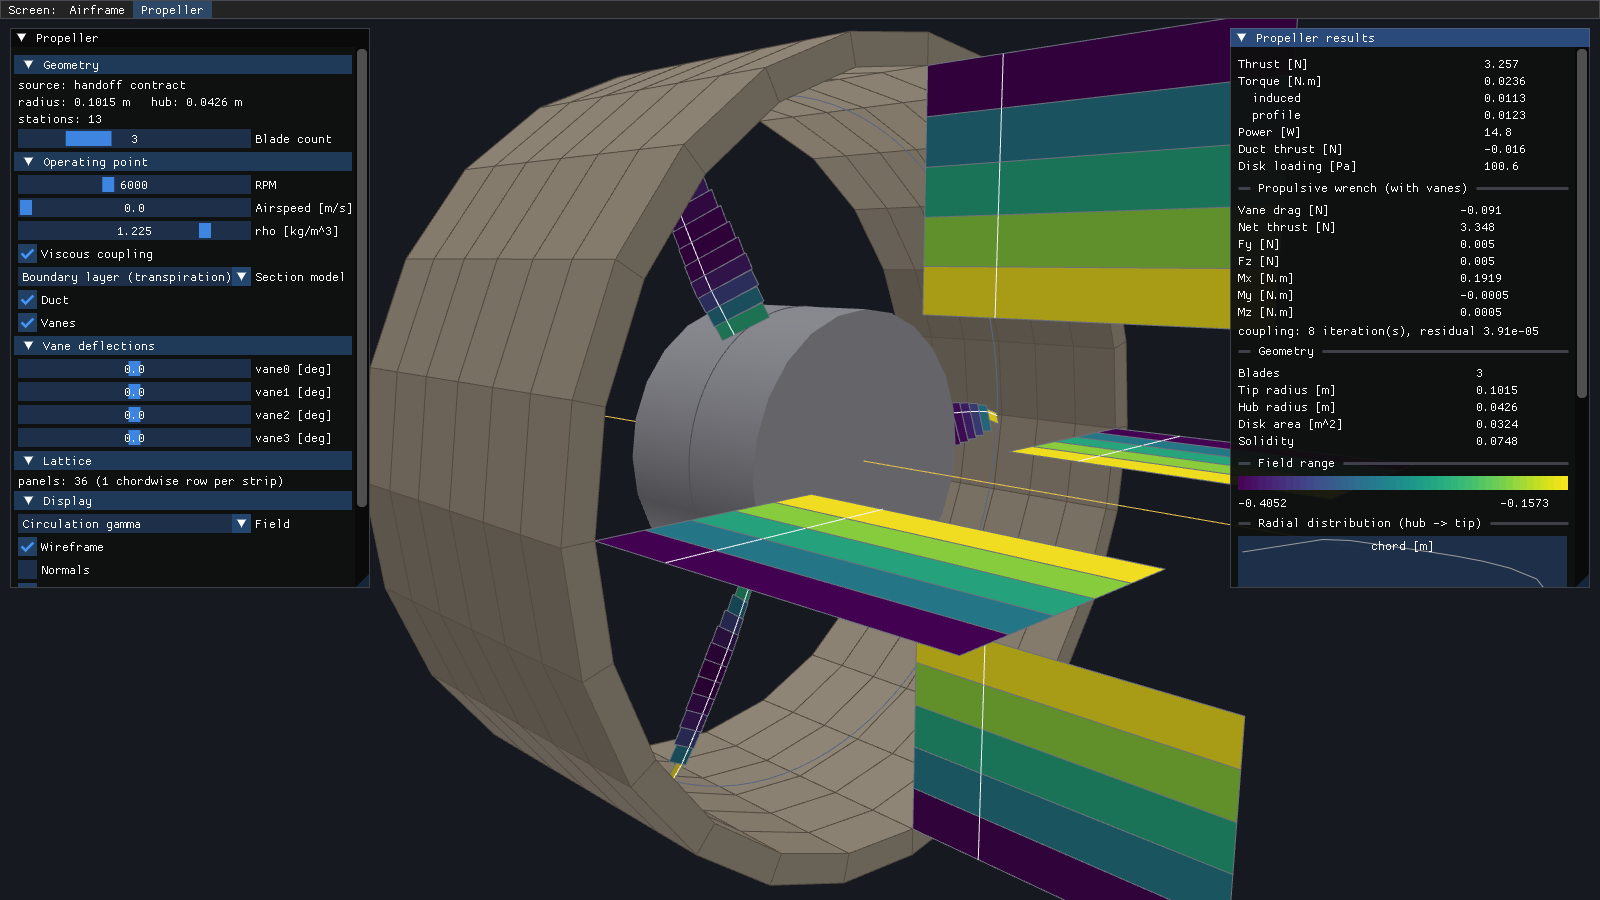
\includegraphics[width=0.48\textwidth]{figures/viewer_vanes_side}
 \caption{The reference configuration: aft view down the bore showing
   the four-vane cruciform around the hub (left), and side view with
   the vane chords running downstream from their exit-plane hinge
   lines (right); blades and vanes colored by solved circulation.}
 \label{f:vanes}
\end{figure}

\paragraph{Verification.} Every claim above is pinned by the automated
test suite: exact cruciform symmetry undeflected, counter-torque
opposing the rotor's, the budget bound $M_x^{vane} \le Q$ at
convergence, opposite commands pulling the wrench opposite ways, drag
cost for commanding against the swirl, and the survival of the
control response under the two-way coupling.
% TODO (journal version): external validation anchors -- published
% ducted-fan / swirl-recovery-vane data or a RANS comparison.

\section{Conclusion}

A ducted fan with exit vanes can be resolved as one coupled
potential-flow system --- rotating-frame vortex lattice for the
blades, source rings for the duct, inertial-frame lifting surfaces for
the vanes reading a momentum-theory slipstream reconstructed from the
solved loading --- with a scalar angular-momentum budget closing the
swirl exchange between the frames. The budget is not a refinement but
a correction of leading order: the unconstrained scheme overpredicted
the recovered vane torque by a factor of three on the reference
configuration, while the coupled scheme converges to the physically
mandated budget-saturated state in a handful of outer passes and
seconds of wall time. The method gives a ducted-fan VTOL designer the
quantities the configuration loop actually needs at hover --- net
thrust with the vanes' drag debit, control moments about the
swirl-biased neutral, and the recovered counter-torque --- from a
parametric geometry description, at interactive speed.

% TODO: futures -- band-resolved swirl budget, vortex-ring wake for
% chordwise loading, forward-flight sweep, external validation.

\section*{Acknowledgments}

% TODO: funding, program, collaborators. AI-assistance disclosure per
% AIAA policy.

\bibliographystyle{aiaa}
\bibliography{references}

\end{document}
